\documentclass[twoside,a4paper]{article}
\usepackage{geometry}
\geometry{margin=1.5cm, vmargin={0pt,1cm}}
\setlength{\topmargin}{-1cm}
\setlength{\paperheight}{29.7cm}
\setlength{\textheight}{25.3cm}

% useful packages.
\usepackage{amsfonts}
\usepackage{amsmath}
\usepackage{amssymb}
\usepackage{amsthm}
\usepackage{enumerate}
\usepackage{graphicx}
\usepackage{multicol}
\usepackage{fancyhdr}
\usepackage{layout}

% some common command
\newcommand{\dif}{\mathrm{d}}
\newcommand{\avg}[1]{\left\langle #1 \right\rangle}
\newcommand{\difFrac}[2]{\frac{\dif #1}{\dif #2}}
\newcommand{\pdfFrac}[2]{\frac{\partial #1}{\partial #2}}
\newcommand{\OFL}{\mathrm{OFL}}
\newcommand{\UFL}{\mathrm{UFL}}
\newcommand{\fl}{\mathrm{fl}}
\newcommand{\op}{\odot}
\newcommand{\Eabs}{E_{\mathrm{abs}}}
\newcommand{\Erel}{E_{\mathrm{rel}}}

\begin{document}

\pagestyle{fancy}
\fancyhead{}
\lhead{Jovi Wong(3180104829)}
\chead{Numerical Analysis homework \#6}
\rhead{2020/5/13}


\section*{I. Convert $477$ to a normalized FPN with $\beta =2$}
We can rewrite this number into $(111011101)_2$, hence $m=1.11011101$ and the normalized binary form is 
\begin{equation}
477=(1.11011101)_2\times2^8
\end{equation}


\section*{II. Convert $\frac{3}{5}$ to a normalized FPN with $\beta=2$}

\begin{equation}
\frac{3}{5}=(0.1001\cdots)_2=(1.00110011\cdots)\times2^{-1}
\end{equation}

\section*{III. Prove $x_R-x=\beta(x-x_L)$}
We can rewrite the condition as  $x=1.0 \times {\beta}^e=(1.0\times\beta)\times\beta^{e-1}$. Additionally, the machine precision is $\epsilon_M=\beta^{1-p}$. Consequently,
\begin{gather}
x_R=(1.0+\beta^{1-p})\times\beta^e \\
x_L=(\beta-\beta^{1-p})\times\beta^{e-1}
\end{gather}
Next step is easy,
\begin{gather}
x_R-x=\beta^{1-p}\times\beta^{e}=\beta^{e-p+1} \\
x-x_L=(\beta\times1.0-\beta+\beta^{1-p})\times\beta^{e-1}=\beta^{e-p}
\end{gather}
Finally, we prove $x_R-x=\beta(x-x_L)$ successfully.

\section*{IV. Find two normalized FPNs adjcent to $x$ and relative roundoff error}
Round off $\frac{3}{5}$ into fl($x$)$=x_R=(1.00110011001100110011010)_2\times2^{-1}$. So the two adjcent normalized FPNs are
\begin{gather}
x_L=(1.00110011001100110011001)_2\times2^{-1} \\
x_R=(1.00110011001100110011010)_2\times2^{-1}
\end{gather} 
As a result, the relateive error is $\epsilon=|\frac{fl(x)-x}{x}|=\frac{2^{-26}+0.6\times2^{26}}{0.6}\approx3.97\times10^{-8}=3.97\times10^{-6}\%$ .

\section*{V. What is the unit roundoff when drop excess bits simply}
\[
\epsilon_u=\epsilon_M=\beta^{1-p}=2^{-23}
\]
\section*{VI. How many bits of precision are lost in $1-\cos{\frac{1}{4}}$}
We can define $fl(a)=1$ and $b=$fl($\cos{\frac{1}{4}}$) by
\begin{gather}
a=M_a\times2^{e_a}=(1.00000000000000000000000)_2\times2^{0} \\
b=M_b\times2^{e_b}=(1.11111111111111101100000)_2\times2^{-1}
\end{gather}
And then define $c=$fl($a-b$)$=M_c\times2^{e_c}$, so 
\begin{gather}
M_c=M_a-\beta^{-1}M_b \\ 
=(1.00000000000000000000000)_2-(0.111111111111111101100000)_2 \\
=(0.000000000000000010100000)_2 \\
=(1.010000000000000000000000)_2\times2^{-17}
\end{gather}
Namely, $c=(1.01000000000000000000000)_2\times2^{-17}$ and 17 bits of precision is lost.

\section*{VII. Suggest two ways to compute $1-\cos{x}$}
Firstly, we can use Taylor series
\begin{gather}
1-\cos{x}=1-(1-\frac{x^2}{2!}+\frac{x^4}{4!}-\frac{x^6}{6!}+\cdots)=\sum_{i=1}^{\infty}(-1)^{i+1}\frac{x^{2i}}{(2i)!}
\end{gather}
Secondly, we can use a trigonometric function formula $\cos{2x}=1-2\sin^2{x}$ such that
\begin{gather}
1-\cos{x}=1-(1-2\sin^2{\frac{x}{2}})=2\sin^2{\frac{x}{2}}
\end{gather}

\section*{C++ programming}
\subsection*{A. Compare three functions}
\begin{figure}[h]
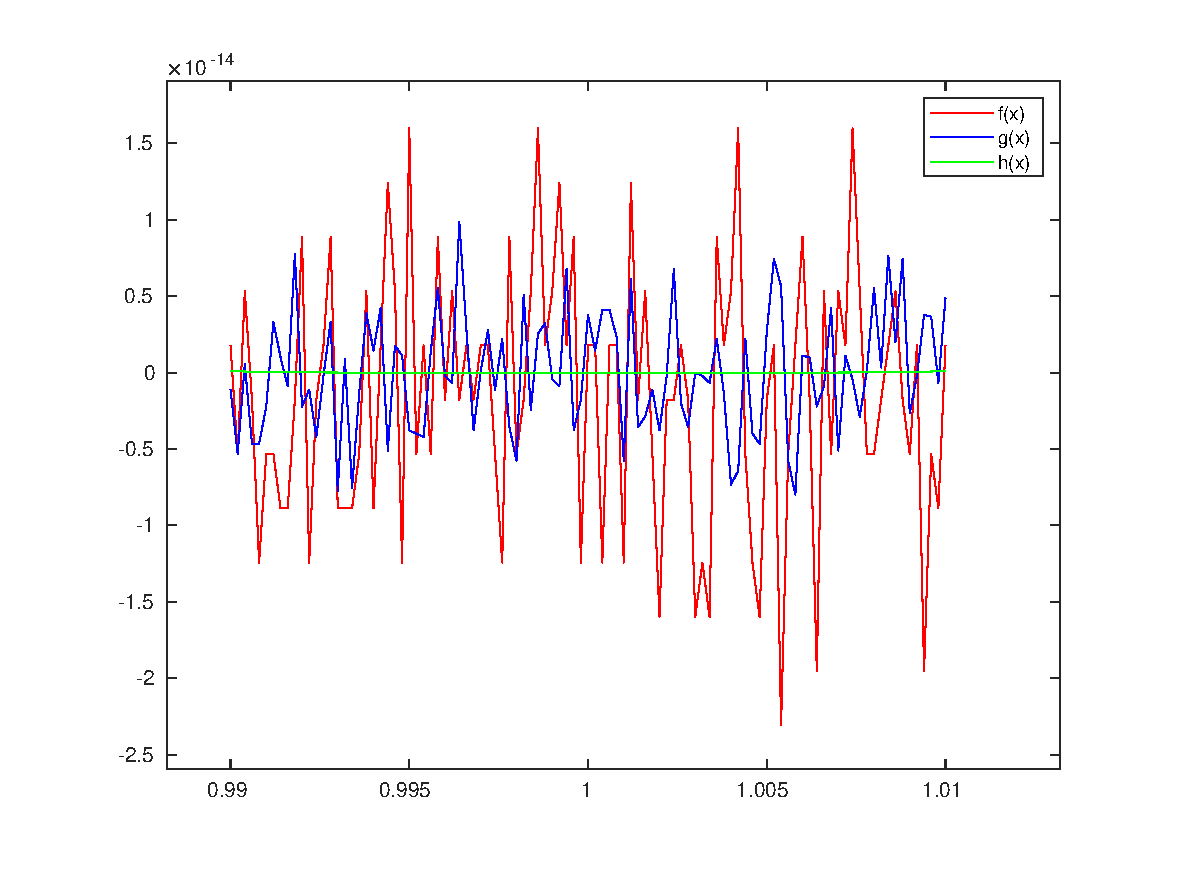
\includegraphics[width=7in]{Figure/comparison.eps}
\caption{the difference between $f(x)$ and $g(x)$ and $h(x)$}
\end{figure}
Multiplication and division are accurate. However, addition, let say $fl(fl(x)+fl(y))$, is not accurate when $x+y\to0$. And function $f(x)$ and $g(x)$ use addition or substraction calculation for eight times but function $h(x)$ uses substraction for only one time. As a result, function $h(x)$ is the most accurate one.

\subsection*{B. Consider a normalized FPN system $\mathbb{F}$}
We can know the $UFL(\mathbb{F})=0.5$ and $OFL(\mathbb{F})=3.5$ easily by definition 1.10. Besides, the enumeration of elements in $\mathbb{F}$ is as following
\begin{gather}
1.00\times2^{-1} , 1.01\times2^{-1} , 1.10\times2^{-1} , 1.11\times2^{-1} \\
1.00\times2^{0} , 1.01\times2^{0} , 1.10\times2^{0} , 1.11\times2^{0} \\
1.00\times2^{1} , 1.01\times2^{1} , 1.10\times2^{1} , 1.11\times2^{1} \\
-1.00\times2^{-1} , -1.01\times2^{-1} , -1.10\times2^{-1} , -1.11\times2^{-1} \\ 
-1.00\times2^{0} , -1.01\times2^{0} , -1.1\times2^{0} , -1.11\times2^{0} \\
-1.00\times2^{1} , -1.01\times2^{1} , -1.1\times2^{1} , -1.11\times2^{1}
\end{gather}
as well as $0$. hence $\#F=2^3\times(1-(-1)+1)+1=25$ consistent with corollary 1.11.
\begin{figure}[h]
\includegraphics[width=8in]{Figure/NumDis1.eps}
\caption{$\mathbb{F}$ on the real axis}
\end{figure}
\\
Additionally, all the subnormal numbers are 0.125 0.25 0.375 -0.125 -0.25 -0.375 . Therefore, the extended $\mathbb{F}$  is as following
\begin{figure}[h]
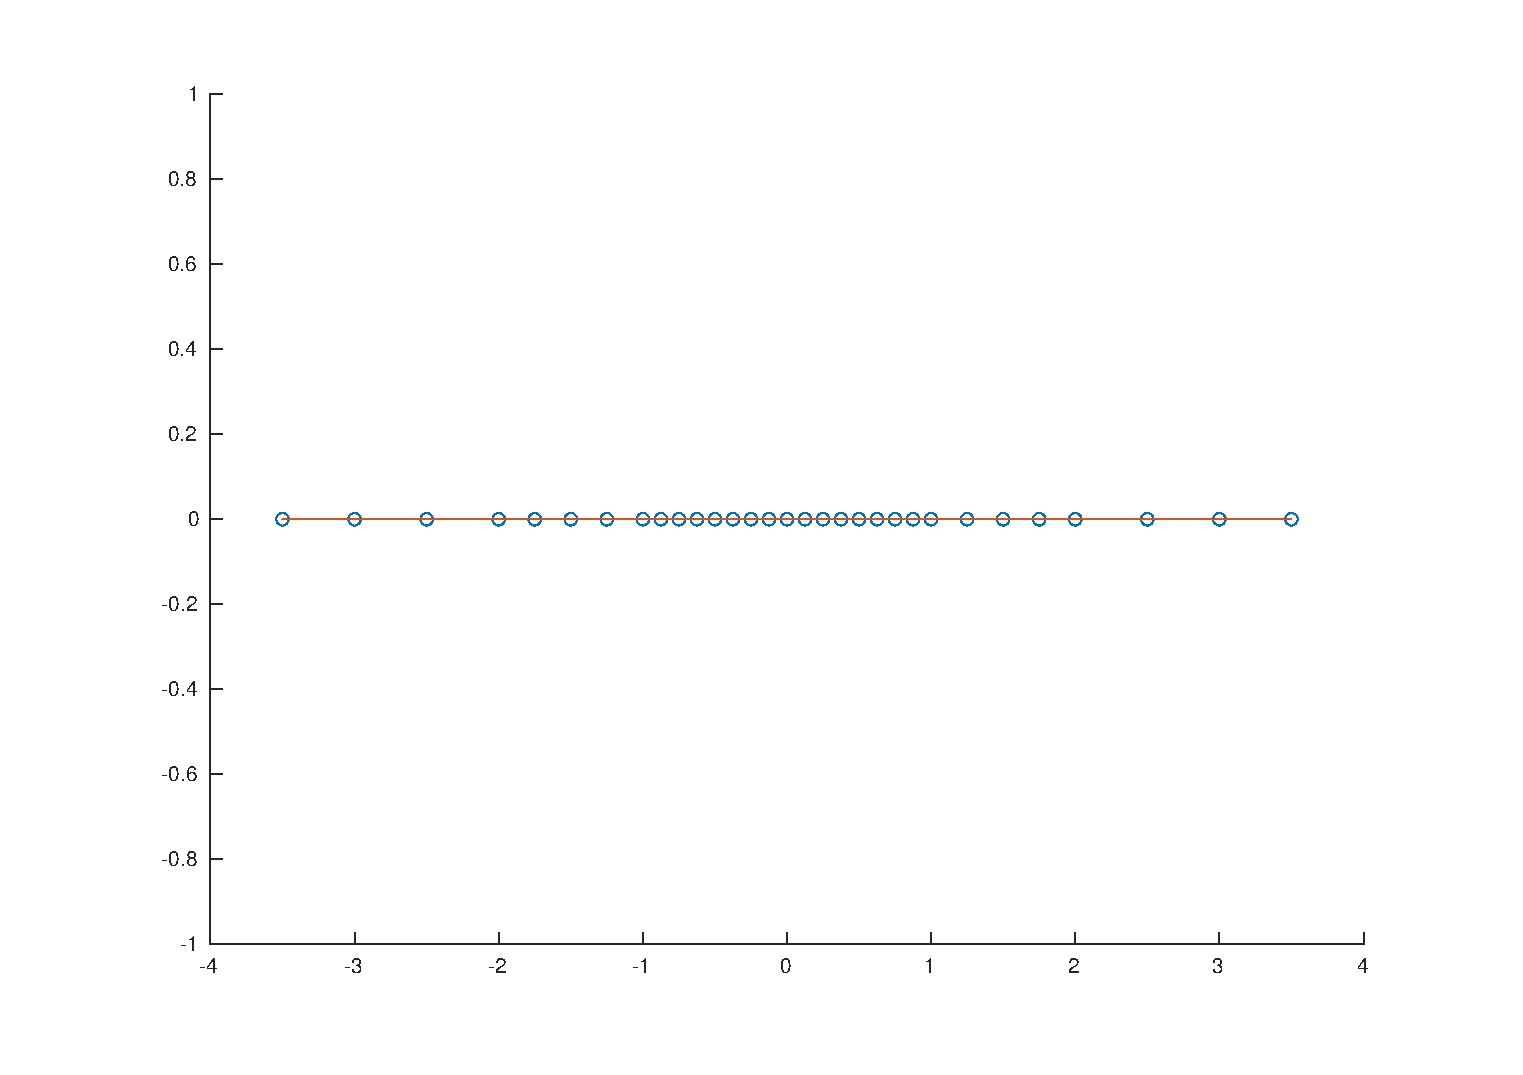
\includegraphics[width=8in]{Figure/NumDis2.eps}
\caption{The $extended$ $\mathbb{F}$ on the real axis}
\end{figure}



\end{document}

%%% Local Variables: 
%%% mode: latex
%%% TeX-master: t
%%% End: 
